
\subsection{Sub-Gaussian Distributions}
The reader may notice that our discussions of concentration inequalities have been restricted to heavy assumptions -- assumptions that random variables are Bernoulli, Symmetric Bernoulli, or bounded. In this section, we will extend our results to a larger class of distributions called the sub-Gaussian distributions. We will then explore its properties.  

% ===============================
% Bounds on Gaussian Distribution
% ===============================
Before we continue further with discussion of Sub-Gaussian distributions, it is worthwhile to explore the bounds on the Gaussian distribution. \\

\begin{tcolorbox}
\begin{proposition}[Tails of the Normal Distribution]
Suppose $X \sim N(0,1)$. For $t > 0$, the tails of the normal distribution may be represented by 
$$ \left(\frac{1}{t} - \frac{1}{t^3} \right) \cdot \frac{1}{\sqrt{2\pi}} e^{-t^2/2} \leq P(X \geq t) \leq \frac{1}{t} \cdot \frac{1}{\sqrt{2\pi}} e^{-t^2/2}$$
\end{proposition}
\end{tcolorbox}

\begin{proof}
\noindent Upper Tail:  \\ 
Strategy: the objective of concentration inequalities is to get the inequalities to be functions of $t$. In other words, we want to get the concentration inequalities to illustrate probabilities as they deviate from the mean. In proofs, we will often simplify expressions using inequalities. However, we never want to simplify any term that includes $t$.    
    \begin{align*}
    P(X \geq t) &= \frac{1}{\sqrt{2\pi}} \int_{t}^{\infty} e^{-x^2/2}dx &&\text{} \\
    &= \frac{1}{\sqrt{2\pi}} \int_{t}^{\infty} e^{-(t+y)^2/2}dy &&\text{change of var: x = t+y} \\
    &= \frac{1}{\sqrt{2\pi}} \int_{t}^{\infty} e^{-t^2/2} e^{-ty} e^{-y^2/2}dy &&\text{} \\
    &= \frac{1}{\sqrt{2\pi}}e^{-t^2/2} \int_{t}^{\infty} e^{-ty} e^{-y^2/2}dy &&\text{since $e^{-t^2/2}$ is not a function of $y$} \\
    &\leq \frac{1}{\sqrt{2\pi}}e^{-t^2/2} \int_{t}^{\infty} e^{-ty}dy &&\text{since $e^{-y^2} < 1$ for $t \in (0, \infty)$ and $y \in [t,\infty)$} \\
    &= -\frac{1}{\sqrt{2\pi}}e^{-t^2/2} \frac{1}{t}e^{-ty}\Bigg|_{t}^{\infty} &&\text{take integral} \\
    &= 0 - \left( -\frac{1}{\sqrt{2\pi}}e^{-t^2/2} \frac{1}{t}e^{-ty} \right) &&\text{} \\
    &= \frac{1}{t} \cdot \frac{1}{\sqrt{2\pi}}e^{-t^2/2} e^{-t^2} &&\text{} \\
    &\leq \frac{1}{t} \cdot \frac{1}{\sqrt{2\pi}} e^{-t^2/2} &&\text{??? Why would we do this} \\
    \end{align*}
\end{proof}

\noindent 
Hoeffding's: $\displaystyle{P\left(\left|\sum_{i=1}^{N} a_i X_i\right| \geq t\right) \leq 2\exp\left( -\frac{t^2}{2 \|a\|_{2}^{2}}\right)}$ \\ 
Chernoff's: $\displaystyle{P\left(\left|\sum_{i=1}^{N}X_i - \mu\right| \geq \delta \mu\right) \leq 2 \exp{\{-c\mu \delta^2\}}}$ \\ 
Normal: $\displaystyle{ P\left(X \geq t \right) \leq \frac{1}{t}\cdot \frac{1}{\sqrt{2\pi}} \exp{\left(-\frac{t^2}{2}\right)} }$ \\ 

Taking a look at the bounds between Hoeffding's inequality and the bound on the normal distribution, there is clearly some similarities. This is a hint that there may be some underlying structure. The notion of sub-Gaussian distributions is a class of distributions where the probabilities in the tails converge at least as fast as the Gaussian distribution. 

To make this even clearer, we may observe that Hoeffding's inequality where $N=1$ results in 
$$ P\left( \left|X \right| \geq t\right) \leq 2\exp\left( -\frac{t^2}{2} \right). $$

\begin{tcolorbox}
\begin{proposition}[Sub-Gaussian Properties]
If $X$ is a random variable, such that $K_1, ..., K_5$ are all positive and are constants, then the following are equivalent 
    \begin{enumerate}
    \item $\displaystyle{ P\left( |X| \geq t \right) \leq 2 \exp\left( -t^2/K_1^2 \right) }$ for $t \geq 0$
    \item $\displaystyle{ \|X\|_{L^p} = \left( E\big[|X|^p\big] \right)^{1/p} \leq K_2\sqrt{p}}$ for $p \geq 1$
    \item The MGF of $X^2$ satisfies
    $$ \Expect{\exponential{\lambda^2 X^2}} \leq \exponential{K_3^2 \lambda^2} $$
    \item The MGF of $X^2$ is bounded at some point. In particular,
    $$ \Expect{\exponential{X^2/ K_4^2}} \leq 2. $$ 
    \item If $E[X] = 0$, then the MGF of $X$ satisfies
    $$ \Expect{\exponential{\lambda x}} \leq \exponential{K_5^2 \lambda^2} for \lambda \in \mathbb{R}$$
    \end{enumerate}
\textbf{Note:} Properties (1)-(5) are equivalent in the sense that there exists some absolute constant $C$, and property $i$ implies property $j$ such that $K_j \leq C K_i. $
\label{prop:subgaussian}
\end{proposition}
\end{tcolorbox}


% ===========
% Add Pictures
% ===========
\begin{figure}[H]
        \centering
        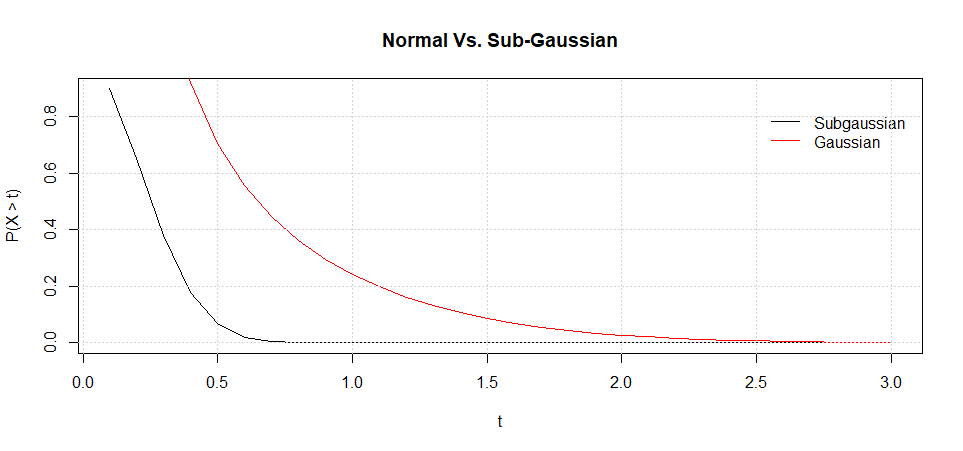
\includegraphics[scale=0.6]{Normal_vs_SubGaussian}
        \caption{Illustration that Sub-Gaussian distributions are \textit{below} the normal distribution -- hence the name. }
\end{figure}

% ============
% Proof 1 => 2
% ============
\begin{proof}
    %%%% 
    $(\text{Property }1 \implies \text{Property }2): $ \textcolor{orange}{Assume (1) is true.} 
    \begin{align*}
    %
    E\big[|X|^p\big] &= \int_{0}^{\infty} P\left(|X|^p \geq u\right)du && 
        \text{Integral Identity $\left(|X|^p \geq 0\right)$} \\ 
    &= \int_{0}^{\infty} \Prob{|X|^p \geq \textcolor{\darkgreen}{t^p} }du &&
        \text{Substitute: $u = t^p$} \\ 
    &= \int_{0}^{\infty} \Prob{ |X|^p \geq t^p }\textcolor{\darkgreen}{pt^{p-1}dt} && 
        \text{$du = pt^{p-1}dt$} \\ 
    &= \int_{0}^{\infty} \Prob{ \textcolor{\darkgreen}{|X| \geq t }}pt^{p-1}dt && 
        \text{$p$th root of both sides} \\ 
    &\leq \int_{0}^{\infty} \textcolor{\darkgreen}{2\exponential{-t^2}}pt^{p-1}dt &&
        \text{Property 1 \textcolor{orange}{assuming $K_1^2=1$}}  \\
    &= p \int_{0}^{\infty} 2t^{p-1} e^{-t^2} dt &&
        \text{Rearrange} \\ 
        %
    \end{align*}
    \textcolor{orange}{Recall} that the Gamma function is 
    \begin{align*}
        \Gamma(z) &= \int_{0}^{\infty} y^{z-1}e^{-y}dy 
            &&\text{defn. } \\ 
        &= \int_{0}^{\infty} \textcolor{\darkgreen}{t}^
            {\textcolor{\darkgreen}{2}(z-1)}e^{-t^2} dy
            &&\text{Substitute $y = t^2$} \\
        &= \int_{0}^{\infty} \textcolor{\darkgreen}{2t} t^{2(z-1)}e^{-t^2} \textcolor{\darkgreen}{dt}
            &&\text{$dy = 2tdt$} \\ 
        &= \int_{0}^{\infty} 2 t^{\textcolor{\darkgreen}{2z - 1}}e^{-t^2} dt
            &&\text{} \\ 
    \end{align*}
    \textcolor{orange}{Continuing on}, and using this representation, we find that 
    \begin{align*}
        \Expect{|X|^p} &\leq p \int_{0}^{\infty} 2t^{p-1} e^{-t^2} dt &&
            \text{From Above} \\ 
        &= p \int_{0}^{\infty} 2t^{\textcolor{\darkgreen}{2(p/2)}-1} e^{-t^2} dt &&
            \text{Rearrange} \\ 
        &= p \cdot \textcolor{\darkgreen}{\Gamma(p/2)} && 
            \text{Gamma Defn.} \\ 
        &\leq p \cdot \textcolor{\darkgreen}{(p/2)^{p/2}} &&
            \text{\textcolor{red}{$\Gamma(x) \leq x^x$ from Stirling Approx.}} \\ 
        \textcolor{\darkgreen}{\big(}\Expect{|X|^p}\textcolor{\darkgreen}{\big)^{1/p}} &\leq \textcolor{\darkgreen}{\big(}(p/2)^{p/2}\textcolor{\darkgreen}{\big)^{1/p}} &&
            \text{take $p$th root of both sides} \\ 
        &= (p/2)^{\textcolor{\darkgreen}{1/2}} &&
            \text{} \\ 
        &= \textcolor{\darkgreen}{K_2} \sqrt{p} && 
    \end{align*}
    %%%% 
\end{proof}

% ==============
% Proof Technique
% ==============
\begin{tcolorbox}[colback=white!90!gray, title=Proof Technique: Bounding $P$-Norm]
\begin{enumerate}
    \item Represent $\Expect{|X|^p}$ with integral identity
    \item Bind $\Expect{|X|^p}$ by sub-Gaussian tail from property 1
    \item Represent exponential tail as Gamma function
    \item Bind Gamma function with $\Gamma(x) \leq x^x$ to create bound dependent only on $p$ 
\end{enumerate}
\end{tcolorbox}


% ==============
% Proof: 2 => 3 
% ==============
\begin{proof}
(Property 2 $\implies$ Property 3): \textcolor{orange}{Assume (2) is true.}
\begin{align*}
M_{X^2}(\lambda^2) &= \Expect{e^{\lambda^2 X^2}} && 
    \text{\textcolor{red}{defn. of MGF of $X^2$} } \\ 
&= \Expect{\textcolor{\dgreen}{\sum_{p=0}^{\infty} \frac{(\lambda^2 X^2)^p}{p!}}} && 
    \text{summation notation of series expansion} \\ 
&= \sum_{p=0}^{\infty} \frac{\lambda^{2p} \textcolor{\dgreen}{\Expect{X^{2p}}}}{p!} &&
    \text{distribute expectation} \\ 
&\leq \sum_{p=0}^{\infty} \frac{ \lambda^{2p} \Expect{X^{2p} } }{\textcolor{\dgreen}{(p/e)^p}} &&
    \text{\textcolor{blue!50!white}{since $(p/e)^p \leq p!$}} 
\end{align*}
Notice that we have 
\begin{align*}
    \Expect{X^{2p}} &= \Expect{\textcolor{\dgreen}{|X|}^{2p}} && 
        \text{since $2p$ is always even} \\ 
    &\leq \left(K_2 \sqrt{2p} \right)^{2p} && 
        \text{$\Expect{|X|^q} \leq \left(K_2 \sqrt{q}\right)^q$ by prop. (2)} \\ 
    &= K_2^{2p} \left(2p \right)^p && 
        \text{} \\ 
    &= (2p)^p && \text{\textcolor{orange}{let $K_2 = 1$}}. 
\end{align*}
Substituting this inequality back into the bound on the MGF, we obtain 
\begin{align*}
    M_{X^2}(\lambda^2) &\leq \sum_{p=0}^{\infty} \frac{ \lambda^{2p} \textcolor{\dgreen}{(2p)^p} }{ (p/e)^p } && 
        \text{substitute $\Expect{X^{2p}} \leq (2p)^p$} \\ 
    &= \sum_{p=0}^{\infty} \textcolor{\dgreen}{(2\lambda^2 e)^p} && 
        \text{} 
\end{align*}
\textcolor{orange}{Recall} that the geometric series states that for $-1 < r < 1$, $\sum_{k=0}^{\infty} r^k = \frac{1}{1-r}.$ It follows now that 
\begin{align*}
    M_{X^2}(\lambda^2) &\leq \textcolor{\dgreen}{\frac{1}{1 - 2\lambda^2 e}} &&\text{ for $-1 < 2\lambda^2 e < 1$} &&& \text{geometric series} \\ 
    & &&\text{ for } \textcolor{\dgreen}{|\lambda| \leq \sqrt{\frac{1}{2e}}} &&&  \\
    &\leq \textcolor{\dgreen}{e^{4 \lambda^2 e}} &&\text{ for $0 \leq 2\lambda^2 e \leq 1/2$} &&& 
        \text{since \textcolor{blue!50!white}{$\frac{1}{1-x} \leq e^{2x}$ for $0 \leq x \leq 1/2$}} \\ 
    & && \text{ for } \textcolor{\dgreen}{|\lambda| \leq \frac{1}{2 \sqrt{e}}}
\end{align*}
\end{proof}

% ==============
% Proof Technique
% ==============
\begin{tcolorbox}[colback=white!90!gray, title=Proof Technique: Bounding MGF of $X^2$]
\begin{enumerate}
    \item represent series expansion of $X^2$ MGF with summation notation 
    \item apply inequalities to bind series expansion of $X^2$ MGF with geometric series
    \item bind geometric series by exponential tail 
\end{enumerate}
\end{tcolorbox}

% =============
% Proof: 3 => 4
% =============
\begin{proof}
(Property 3 $\implies$ Property 4): \textcolor{orange}{Assume (3) is true}.
We know that 
\begin{align*}
    \Expect{\lambda^2 \exponential{X^2}} &\leq \exponential{K_3^2 \lambda^2} && |\lambda| \leq \frac{1}{K_3} &&& \text{Prop. 3} \\
    & && \lambda^2 \leq \frac{1}{K_3^2} &&&  \\
    \implies \Expect{\exponential{X^2/\textcolor{\dgreen}{K_3^2}}} &\leq \exponential{K_3^2 / \textcolor{\dgreen}{K_3^2}} = e && &&& \text{for $\lambda^2 = 1/K_3^2$} 
\end{align*}
If we choose a $K_4 > K_3$, then the tail is bounded even further.  \\ 
\end{proof}

% ============
% Proof 4 => 1
% ============
\begin{proof}
(Property 4 $\implies$ Property 1): \textcolor{orange}{Assume (4) is true and $K = 1$}. It follows that 
\begin{align*}
    \Prob{|X| \geq t} &= \Prob{|X^{\textcolor{\dgreen}{2}}| \geq t^{\textcolor{\dgreen}{2}}} && 
        \text{square both sides} \\ 
    &= \Prob{\textcolor{\dgreen}{e}^{x^2} \geq \textcolor{\dgreen}{e}^{t^2}} &&
        \text{exponentiate both sides} \\ 
    &\leq \frac{E[\textcolor{\dgreen}{e}^{x^2}]}{\textcolor{\dgreen}{e}^{t^2}} &&
        \text{Markov's Inequality} \\ 
    &\leq 2e^{-t^2} &&
        \text{Property 4: $E[e^{x^2/k^2}] \leq 2$}
\end{align*}
\end{proof}

% ==============
% Proof Technique
% ==============
\begin{tcolorbox}[colback=white!90!gray, title=Proof Technique: Bounding Tail Decay]
\begin{enumerate}
    \item bound MGF with Markov's Inequality
    \item Apply MGF boundedness property to bound tail decay
\end{enumerate}
\end{tcolorbox}


% =============
% Proof 3 => 5 
% =============
\begin{proof}
(Property 3 $\implies$ Property 5): \textcolor{orange}{Assume (3) is true.}  \\ 


\noindent Case 1:$|\lambda| \leq 1$. \\
\noindent Notice that \textcolor{\lblue}{$e^x \leq x + e^{x^2/2}$ for all $x \in \mathbb{R}$}. It follows that 
\begin{align*}
    \Expect{e^{\lambda X}} &\leq \Expect{\lambda X + \exponential{\lambda^2 X^2 / 2}} &&
        \text{$e^x \leq x + e^{x^2/2}$} \\ 
    &= \lambda \Expect{X} + \Expect{\exponential{\lambda^2 X^2 /2 }} && 
        \text{distribute expectation} \\ 
    &= 0 + \Expect{\exponential{\lambda^2 X^2 /2 }} && 
        \text{since $E[X] = 0$ by hypothesis} \\ 
    &\leq \exponential{K^2 \lambda^2} && 
        \text{Property 3}
\end{align*}

\noindent Case 2: $|\lambda| \geq 1$.  \\
\noindent Notice that \textcolor{\lblue}{$2\lambda x \leq \lambda^2 + x^2$ for all $x \in \mathbb{R}$}. Under further analysis, we have 
\begin{align*}
2\lambda x &\leq \lambda^2 + x^2  \\
\implies e^{\lambda x} &\leq e^{\frac{\lambda^2 + x^2}{2}}. 
\end{align*}
It follows that 
\begin{align*}
    \Expect{e^{\lambda X}} &\leq \Expect{e^{\frac{\lambda^2+X^2}{2}}} && 
        \text{$2\lambda x \leq \lambda^2 + x^2$} \\ 
    &= e^{\lambda^2/2} \Expect{e^{X^2/2}} \\ 
    &\leq e^{\lambda^2/2} \textcolor{\dgreen}{e^{1/2}} &&\text{Prop. 3: $\Expect{e^{\lambda x}} \leq e^{1/2}$ for $K=1$} \\ 
    &= e^{\frac{\lambda^2+1}{2}} && \text{} \\ 
    &\leq e^{\lambda^2} && \text{$\lambda \geq 1 \implies \lambda^2 \geq 1 \implies$} \\ 
    & && \text{$\lambda^2+1 \geq 2 \implies  \frac{\lambda^2+1}{2} \geq 1$}
\end{align*}
\end{proof}

\begin{figure}[H]
\begin{subfigure}{0.5\textwidth}
    \centering
    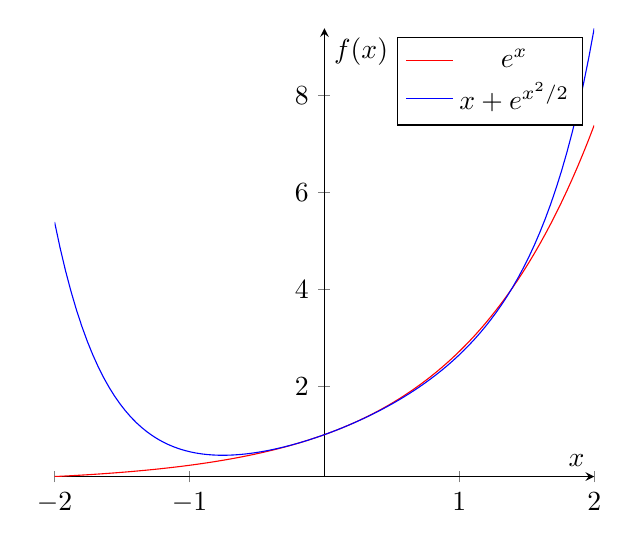
\begin{tikzpicture}
    \begin{axis}[
        axis lines = center,
        xlabel = $x$,
        ylabel = {$f(x)$},
    ]
    %Below the red parabola is defined
    \addplot [
        domain=-2:2, 
        samples=100, 
        color=red,
    ]
    {e^x};
    \addlegendentry{$e^x$}
    %Here the blue parabloa is defined
    \addplot [
        domain=-2:2, 
        samples=100, 
        color=blue,
        ]
    {x + exp(x^2/2)};
    \addlegendentry{$x + e^{x^2/2}$}
    \end{axis}
    \end{tikzpicture}
\end{subfigure}
\begin{subfigure}{0.5\textwidth}
    \centering
    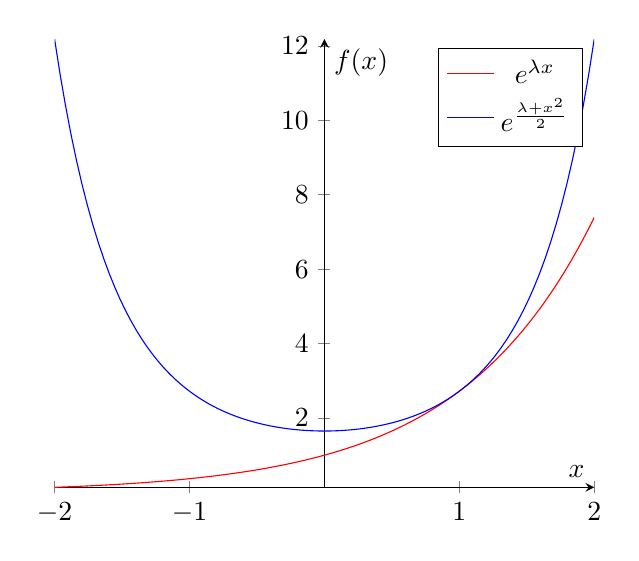
\begin{tikzpicture}
    \begin{axis}[
        axis lines = center,
        xlabel = $x$,
        ylabel = {$f(x)$},
    ]
    %Below the red parabola is defined
    \addplot [
        domain=-2:2, 
        samples=100, 
        color=red,
    ]
    {exp(x)};
    \addlegendentry{$e^{\lambda x}$}
    %Here the blue parabloa is defined
    \addplot [
        domain=-2:2, 
        samples=100, 
        color=blue,
        ]
    {exp(1/2+x^2/2)};
    \addlegendentry{$e^{\frac{\lambda + x^2}{2}}$}
    \end{axis}
    \end{tikzpicture}
\end{subfigure}
\end{figure}




% ==============
% Proof: 5 => 1 
% ==============
\begin{proof}
(Property 5 $\implies$ Property 1): \textcolor{orange}{Assume (5) is true and $E[X]=0.$}
\begin{align*}
    \Prob{X \geq t} &= \Prob{e^{\lambda x} \geq e^{\lambda t}} && \text{} \\
    &\leq \textcolor{\dgreen}{e^{-\lambda t} \Expect{e^{\lambda x}}} &&
        \text{Markov's Inequality} \\ 
    &\leq e^{-\lambda t} \textcolor{\dgreen}{\exponential{K^2 \lambda^2}} &&
        \text{Prop. 5: $\Expect{e^{\lambda x}} \leq \exponential{K^2 \lambda^2}$} \\ 
    &= \exponential{K^2 \lambda^2 - \lambda t} 
\end{align*}
Now, optimizing the bound to obtain the smallest upper bound, we have 
\begin{align*}
    \frac{d}{d \lambda} \left(\exponential{-\lambda t + K^2 \lambda^2 }\right) &= \exponential{-\lambda t + K^2\lambda^2} \left( -t + 2K^2 \lambda \right) && \text{product rule} \\  
    \implies 2 \lambda K^2 \exponential{-\lambda t + K^2 \lambda} &= t \exponential{-\lambda t + K^2 \lambda} \\ 
    \implies 2 \lambda K^2 &= t   \\
    \implies \lambda &= t/2K^2 \\ 
    \implies \lambda &= t/2 && \text{\textcolor{orange}{Let K =1}}
\end{align*}
Plugging $\lambda$ back into the bound, we obtain
\begin{align*}
    \Prob{X \geq t} &\leq \exponential{\textcolor{\dgreen}{t^2/4 - t^2/2}} && \text{$\lambda = t/2$} \\ 
    &= \exponential{-t^2/4} \\
    &= \exponential{-t^2/K^2} && \text{for $K = 2$} 
\end{align*}
\end{proof}

\begin{tcolorbox}
\begin{example}[Property 5 without 0 Mean]
Show that Property 5 does not hold if $E[X] \neq 0.$ \\ 
\end{example}
\end{tcolorbox}
\begin{proof}
\textcolor{orange}{Assume that Property 3 holds. } 
\begin{align*}
    \Expect{e^{\lambda X}} &\leq \Expect{\lambda X + e^{\lambda^2 X^2}} && 
        \text{$e^x \leq x + e^{x^2}$} \\ 
    &= \lambda \Expect{X} + \Expect{e^{\lambda^2 X^2}} && \text{} \\
    &\leq \lambda \Expect{X} + \exponential{\lambda^2 K^2}
\end{align*}
Since $\lambda \geq 0$, and $E[X] \neq 0$, for the case that $E[X] < 0$, the bound will be tighter than it should be. Also notice, that we cannot change the value of $K$ because $K$ is related to the absolute constant $C$, which is unchanging. 
\end{proof}



% Definition: Sub-Gaussian Random Variables
\begin{tcolorbox}
\begin{definition}[Sub-Gaussian Random Variable]
A random variable is said to be \textit{sub-gaussian} if it satisfies one of the four properties in Proposition \ref{prop:subgaussian}. Furthermore, we define the sub-gaussian norm as 
    \begin{equation}
    \|X\|_{\psi_2} = \inf\left\{ t>0: \Expect{\exponential{X^2/t^2}} \leq 2 \right\} \\
    \end{equation}
\end{definition}
\end{tcolorbox}

The properties in Proposition \ref{prop:subgaussian} \textit{feel} arbitrary because of the $K$ constants. There exists some absolute constant $C$ that relates all of the $K$ constants together, but the inequalities posed in Proposition \ref{prop:subgaussian} do not illustrate this connection. However, it turns out that we can rewrite the properties in terms of the sub-gaussian norm, resulting in more expressive forms -- illustrating the underlying relationship with $C$: \\ 

\begin{tcolorbox}[colback=white!90!gray, title=Proposition \ref{prop:subgaussian} With Sub-Gaussian Norm]
For $c>0$, and $C$ an absolute constant, 
    \begin{align}
    \Prob{|X| \geq t} &\leq 2 \exponential{-ct^2 / \|X\|^2_{\psi_2}} &&\text{ for $t\geq 0$} \\ 
    \|X\|_{L_p} &\leq C \|X\|_{\psi_2} \sqrt{p} &&\text{ for $p \geq 1$} \\ 
    \Expect{\exponential{X^2 / \|X\|^2_{\psi_2}}} &\leq 2  \\ 
    \text{if $E[X]=0$, } \Expect{\exponential{\lambda X}} &\leq \exponential{\left(C \lambda^2 \|X\|_{\psi^2}^{2} \right)} && \text{ for $\lambda \in \mathbb{R}$}
    \end{align}
\end{tcolorbox}

